% body.tex -- shared by main.tex (IEEEtran, for Overleaf) and preview.tex (local stand-in build).
% Every number below is either a \N... macro (generated from results/ by scripts/make_paper_numbers.py)
% or is attributed to a cited, verified source.

\begin{abstract}
Fake references are difficult to catch because they resemble real ones. It has been argued in the author’s
literature review that format inspection alone cannot therefore distinguish real from fabricated references,
and that detection must be based in a bibliographic database.This paper tests the computational piece of that argument
in a small, fully offline, controlled simulation.We consider a closed-world index of \NnKept{} real records from a
personal bibliography. We then generate true references and three families of defective references (invented, 
chimeric, perturbed-real) and compare four verifiers under a frozen protocol: two format-only methods, a title-only
lookup, and a full-field database consistency check.Format-only verifiers sit at chance (AUROC \NVoneRAuroc{} for the
learned classifier) with a format-faithful fabricator, only gaining signal as the fabricator becomes sloppier (AUROC
\NVoneAurocHigh{} at a 50\% malformation rate). A title-only lookup finds invented titles (recall \NVthreeFone{})
but almost never chimeric ones (\NVthreeFtwo{}). The full-field check achieves recall \NVtwoRRec{} at a 5\% false-positive
rate, but its false-positive rate follows index incompleteness (\NVtwoFprHalf{} at 50\% coverage), so at an assumed 2\% 
prevalence its positive predictive value falls from \NVtwoPpv{} to \NVtwoPpvHalf{}.Perturbed-real references are hardest 
(recall \NVtwoFthree{} on average, ranging \NfthreeMin{}--\NfthreeMax{} across seeds), which we attribute, post hoc, 
to the interaction between the false-positive budget and benign typing noise. All results are for the simulation, not
for language-model output or human readers; several are a consequence of the design, as we explicitly state.
\end{abstract}

\begin{IEEEkeywords}
citation verification, fabricated references, hallucination detection, controlled simulation, reproducibility
\end{IEEEkeywords}

\section{Introduction}
Large language models can produce citations with realistic authors, titles, venues and years which refer to non-existent works.
Walters and Wilder manually inspected 636 citations in ChatGPT produced literature reviews and found that 55\% (GPT-3.5)
and 18\% (GPT-4) were completely fabricated \cite{walters2023}. In an accompanying review I synthesised reasons for why
these references are believed. They are believed due to their reference format which provide a secondary signal for authority,
and rarely being verified. The review concluded with two computational claims which could not be verified computationally. (i)
Fabricated references are presented correctly so they \emph{format inspection alone} cannot be identified through their format. 
(ii) Fabricated references can only be confirmed \emph{exists} to exist using automated matching. This means they cannot be confirmed to be 
consistent with the reference \emph{as written} they are presented as. This requires verification from a database.This paper turns
those claims into measurable questions. It is a controlled comparative study (a ``Pathway B'' study in the course
taxonomy), not a new algorithm, and we make \emph{no claim of novelty}: citation-verifier benchmarks already exist, notably HALLMARK
\cite{reizinger2026} and CiteTracer \cite{li2026}. Our contribution is a small, offline, fully reproducible study that isolates three
variables those benchmarks mix together: how much signal \emph{format} carries when fabrications are format-faithful, what a
\emph{title-only} lookup adds over a \emph{full-field} check, and how both degrade when the reference database is incomplete.


\textbf{Research questions.}  \textbf{RQ1:} When fake references mimic real ones in terms of formatting, how effective
are format-only signals in detecting them? RQ2: For each fabrication family, what is the performance
of title-only checks and full-field consistency checks in terms of what is detected and missed?
RQ3: What is the behaviour in cases where only a subset of real references are indexed? What are
the implications in terms of true positives proportion at realistic prevalence?


\textbf{Scope and honesty statement.} The fabrications are explicitly generated according to a set of rules. 
It is using an index (not Crossref) which contains a closed-world bibliography. We make no claims about trust with humans. 
Threats to validity can be found in Section~\ref{sec:threats}.


\section{Background and Related Work}
\subsection{What the review established}
Figure~\ref{fig:loop} replicates the explanation given in the review for why fake references are trusted. They have superficially
credible characteristics which act as peripheral cues. These cues allow fluent processing and prevent systematic checking.
Table~\ref{tab:review} summarises the statistical findings of the review. The percentage range given by Khurana et al (35-77%) was
listed in the review draft as the ``error rate''. This however, refers to the hallucination rate when language models are asked
to judge claims. It is therefore a measurement of the language model behaviour rather than the proportion of fake references. This has been corrected in Table~\ref{tab:review}. The percentages in Table~\ref{tab:review} have also been verified using the abstracts or pages of the sources used during this project.

\begin{figure}[t]
\centering
\begin{tikzpicture}[
  box/.style={rectangle, draw=blue!60!black, fill=blue!5, rounded corners, thick, align=center,
              text width=5.6cm, font=\scriptsize, inner sep=3pt},
  arr/.style={-Stealth, thick, color=blue!70!black}, node distance=0.42cm]
\node (a) [box] {\textbf{AI-generated text}\\contains a fabricated but perfectly formatted citation};
\node (b) [box, below=of a] {\textbf{Peripheral authority cue}\\plausible authors, year, journal name, DOI};
\node (c) [box, below=of b] {\textbf{Cognitive fluency}\\reader bypasses systematic verification};
\node (d) [box, below=of c] {\textbf{Unearned trust}\\false claim is accepted as credible};
\draw[arr] (a)--(b); \draw[arr] (b)--(c); \draw[arr] (c)--(d);
\end{tikzpicture}
\caption{The heuristic-processing loop for fabricated citations, as argued in the author's review.
This is the motivating hypothesis; the present study does \emph{not} test human readers.}
\label{fig:loop}
\end{figure}

\begin{table*}[t]
\caption{Citation-fabrication evidence from the review, restated with what each study actually measured (verified against primary sources).}
\label{tab:review}
\centering\footnotesize
\begin{tabular}{@{}p{3.1cm}p{4.2cm}p{4.4cm}p{4.8cm}@{}}
\toprule
Study & Systems / sample & Quantity measured & Reported value \\
\midrule
Walters \& Wilder \cite{walters2023} & ChatGPT-3.5 and -4; 636 citations in 84 papers & Citations entirely fabricated & 55\% (GPT-3.5); 18\% (GPT-4) \\
Cabezas-Clavijo \& Sidorenko-Bautista \cite{cabezas2025} & Eight consumer chatbots & Reference fully correct; flawed or fabricated & 26.5\% fully correct; $\approx$40\% flawed or fabricated \\
Khurana et al.\ \cite{khurana2026} & Seven LLMs; 220{,}564 prompts; four domains & \emph{Model} hallucination rate on claim-judgement prompts (not a rate of fabricated references) & Up to 35--77\% (general knowledge) when a fabricated citation accompanies a true claim; +3 to $>$22 pp over a no-citation baseline \\
Liu et al.\ \cite{liu2026} & U.S.\ court filings & Filings containing AI-fabricated citations (a count) & Over 1{,}000; growing year over year \\
\bottomrule
\end{tabular}
\end{table*}

\subsection{Citation-verification benchmarks}
HALLMARK \cite{reizinger2026} comprises 2,526 BibTeX examples grouped into 14 hallucination categories and 3 difficulty levels. It
shows how well a DOI lookup baseline, state-of-the-art LLMs, tool-assisted agents, and a rule-based verification method work.
The abstract says that the false positive rates (rather than recall) impact whether the verifications flagged are predominantly correct or
noise. CiteTracer \cite{li2026} uses a fine-grained 12-code taxonomy, artificial data set of 2,450 citations, and a multi-agent detection
system. However, Aslett et al. have shown that performing an online search to verify claims can increase belief in the claim for
news \cite{aslett2024}. Our simulation is much simpler and smaller than these benchmarks but provides a complimentary test by isolating the
impact of format, title only matching, and index coverage.

\section{Hypotheses and Decision Rules}
Hypotheses and numerical criteria were formulated and hashed in advance of running (Section~\ref{sec:protocol}).
\textbf{H1:} Learned format-only classifier produces an AUROC in the range [0.45, 0.60] when using a format faithful fabricator.
\textbf{H1b:} This AUROC increases by at least 0.15 when varying the malformation rate of the fabricator between 0.05 and 0.50.
\textbf{H2:} Full field search will achieve a recall of $\geq$0.85 at a 5% FPR, with a complete index.
\textbf{H3:} Title only search will achieve a recall of $\leq$0.20 on chimeric references and all non-title perturbations.
\textbf{H4:} Full field search will have an FPR of within 0.05 of $(1-c)+0.05c$ when the full coverage threshold is held constant, with an index coverage of $c$.
A development run was carried out to check if there were any issues, using a separate unreported seed. As a result the thresholds are known values and therefore not guesses. Two issues were found during the initial run and fixed (Section~\ref{sec:deviations}).

\section{Method}
\subsection{Corpus and index}
The file is called frankenstein.bib \cite{swift} and is included in TeX Live. The bibliography contains $ \NnRaw $ entries, $\NnKept$ of which are valid (after 
deduplication), containing author, title, 4-digit year and journal name (articles only). Of these, there are: $ \NnBook $ books, $ \NnArticle $
articles, $ \NnOther $ chapters/proc. papers with years between $\NyearMin$-$\NyearMax$. Since all entries in this bibliography are assumed to be
real works (since it is considered as the researchers library, although we were unable to confirm this independently), they are all valid. As there was no
licence given for this file, only the SHA-256 hash and build script are stored in the repository.



\subsection{Candidate generation}
For the generator we produce one candidate from each class for each indexed record (Fig.~\ref{fig:pipeline}):
G (genuine): The indexed record but with benign noise added.
F1 (fabricated): Authors are recombined from different name pools. Title is a word-bigram chain, not present in any indexed titles with a similarity score of above 0.9. Venue, Publisher and Numbers are taken from a randomly selected donor.
F2 (chimeric): Metadata from record A. Title from record B.
F3 (perturbed genuine): One field has been changed from an indexed record. Year $\pm$1--5, surname of an author, one word in title, journal, publisher, volume and/or pages. This reflects issues reported of incorrect years, volumes and pages \cite{walters2023}.
Benign noise are alterations such as: adding initials, removing optional fields, typos in title, title in sentence case, and removing subtitle. This was added to all four classes at the same rate. Format corruption were corrupting of: year, pages, venue, author, and title. These were added to each field at a rate of $\rho_g{=}0.05$ for the genuine records and $\rho_f\in\{0.05,0.25,0.50\}$ for the faulty records. $\rho_f{=}\rho_g$ is when no format corruption has been applied (format faithful). This simulation reflects mechanisms that have been reported in the literature but does not reflect any particular model's outputs.

\begin{figure}[t]
\centering
\begin{tikzpicture}[
  bx/.style={rectangle, draw=blue!60!black, fill=blue!5, rounded corners, thick, align=center,
             font=\scriptsize, inner sep=3pt, text width=3.3cm, minimum height=0.95cm},
  arr/.style={-Stealth, thick, color=blue!70!black}]
\node[bx] (a) at (0,0) {\textbf{1. Index}\\\NnKept{} real records};
\node[bx] (b) at (4.0,0) {\textbf{2. Generator}\\G, F1, F2, F3 + benign noise + malformation ($\rho_g,\rho_f$)};
\node[bx] (c) at (4.0,-2.05) {\textbf{3. Verifiers}\\V0 random, R1 rule, V1 format LR, V3 title-only, V2 full-field};
\node[bx] (d) at (0,-2.05) {\textbf{4. Evaluation}\\grouped 5-fold CV; $\tau$ at 5\% FPR from training folds};
\draw[arr] (a)--(b); \draw[arr] (b)--(c); \draw[arr] (c)--(d);
\draw[arr, dashed] (a.south) -- ++(0,-0.35) -| ([xshift=-0.9cm]c.north) node[pos=0.28, above, font=\tiny] {index lookup (V2, V3)};
\end{tikzpicture}
\caption{Experimental pipeline. Variants of one source record always share a cross-validation fold (no leakage).}
\label{fig:pipeline}
\end{figure}

\subsection{Verifiers}
\textbf{V0} randomly scores. R1 naively scores references that appear to be valid (year, no raw et al., no all capital title,
valid page information etc.). V1 is a logistic regression model with \NnFeat{} L2 features based on structural
information (counts, valid, present and type). The index and lexical title information is never seen. V3 gets the
top five titles from the index using character TF-IDF and ranks them according to the most similar title (existential). V2 ranks the
candidates using a static weighted score (title 0.40, authors 0.30, year 0.10, venue/publisher 0.10, volume/pages 0.10). This score takes
into account how many fields there are by renormalising. V2 and V3 are simplifications to simulate cross referencing of a database. They are
not copies of any published tools.

\subsection{Protocol and metrics}\label{sec:protocol}
There are 5 seeds (0-4), all of which retrain all candidates and folds. Folds are organised in groups according to their source
record (variant of a record will never be split between training and test). All operational thresholds are set to the 5th (or 95th)
percentile of real training scores meaning that each verifier has a 5% target FPR independent of test data. The primary metric is
out-of-fold recall of faulty references using these thresholds. Secondary metrics are mean recall across folds, family specific
recall and PPV at an assumed 2% prevalence. These are calculated using $\mathrm{PPV}=\frac{r\,\pi}{r\,\pi+f\,(1-\pi)}$ where recall = $r$,
FPR = $f$ and prevalence = $\pi{=}0.02$. During the coverage sweep, a random proportion of $c$
index records are excluded. Thresholds are not changed, they remain as in the full coverage experiments. The average result +/- $\pm$
SD is given. No significance tests were conducted. The protocol file and hash was fixed prior to running.

\subsection{Reproducibility}
We ran the experiments using Python 3.12.3, scikit learn 1.8.0 [pedregosa2011], numpy 2.4.4, pandas 3.0.2, using one CPU core. All seeds and fidelities were run for around 2 minutes (python scripts/run_experiments.py). Figures and tables were created from these saved CSVs. No data was written manually.

\section{Baseline Validation}
On a non-reported seed we verified that behaviour was identical; when records were duplicated exactly in \NnKept{} then V2
and V3 both give scores of 1.0, and always return the correct record. Candidate generation is deterministic at the bit level,
groups do not overlap between folds, and models trained on shuffled labels with V1 have an average AUROC score of \NvalPermMean{}
(over five shuffles between \NvalPermMin{} and \NvalPermMax{}). When one field was changed in a clean probe the score for V2 dropped by
\NvalDropYear{} (year; 0.10), \NvalDropAuthor{} (first author; 0.30) and \NvalDropVenue{} (venue/publisher; 0.10). The last value is less due to partial fuzzy scoring
still being applied when the venue string is different. This is a limitation of V2. Finally all twelve unit tests passed. Three of these
are regression tests as they were added after two defects (D1 and D2) were found (see Section~\ref{sec:deviations}) which had not been
covered by the original nine tests.

\section{Results}
\subsection{Main comparison (RQ1, RQ2)}
The main results for the format-faithful scenario are shown in table~\ref{tab:main}.
V2 achieved a recall of \NVtwoRRec{} with an FPR of \NVtwoRFpr{} (AUROC=\NVtwoRAuroc{}). V3 achieved a recall of \NVthreeRRec{} while both the format only approaches performed at chance (V1 AUROC=\NVoneRAuroc{}, R1 AUROC=\NRoneAuroc{}). This means that R1 achieved the recall by highlighting \NRoneFpr{} real references.
The actual FPR achieved by V1 was higher than the 5\% target (\NVoneRFpr{}), meaning that thresholding does not perfectly generalise between training and testing.

\begin{table*}[t]
\caption{Main comparison, format-faithful fabricator ($\rho_f{=}0.05$), complete index. Mean $\pm$ SD over 5 seeds. FPR is on genuine references; R-F1/F2/F3 are recall per defective family at the operating point; PPV assumes 2\% prevalence.}
\label{tab:main}
\centering\footnotesize
\begin{tabular}{@{}lccccccc@{}}
\toprule
Verifier & AUROC & FPR & Recall & R-F1 & R-F2 & R-F3 & PPV@2\% \\
\midrule
V0 random & 0.508$\pm$0.015 & 0.051$\pm$0.001 & 0.050$\pm$0.010 & 0.05$\pm$0.01 & 0.05$\pm$0.01 & 0.05$\pm$0.02 & 0.020 \\
R1 well-formed rule & 0.497$\pm$0.006 & 0.228$\pm$0.008 & 0.223$\pm$0.005 & 0.22$\pm$0.02 & 0.24$\pm$0.01 & 0.21$\pm$0.02 & 0.020 \\
V1 format-only LR & 0.504$\pm$0.016 & 0.085$\pm$0.013 & 0.089$\pm$0.016 & 0.09$\pm$0.02 & 0.09$\pm$0.02 & 0.09$\pm$0.02 & 0.022 \\
V3 title-only lookup & 0.693$\pm$0.006 & 0.038$\pm$0.008 & 0.406$\pm$0.012 & 0.95$\pm$0.02 & 0.04$\pm$0.01 & 0.23$\pm$0.02 & 0.183 \\
V2 full-field check & 0.985$\pm$0.002 & 0.052$\pm$0.004 & 0.918$\pm$0.070 & 1.00$\pm$0.00 & 1.00$\pm$0.00 & 0.76$\pm$0.21 & 0.267 \\
\bottomrule
\end{tabular}
\end{table*}

Fig.~\ref{fig:family} and Table~\ref{tab:f3} illustrate where verifiers succeed. The title-only strategy performs very well with fake references
(see \NVthreeFone{}) but cannot distinguish chimeric references (see \NVthreeFtwo{}) since these have a genuine title. It also fails to detect any perturbation
apart from those to the title. However, full-field verification detects both fake and chimeric references almost all of the time (see \NVtwoFone{}, \NVtwoFtwo{})
but does not detect many of the perturbed real references. This includes single word changes to the title (see \NVtwoSubTitle{}) and changes to the venue/publisher (see \NVtwoSubVenue{}).

\begin{figure}[t]
\centering
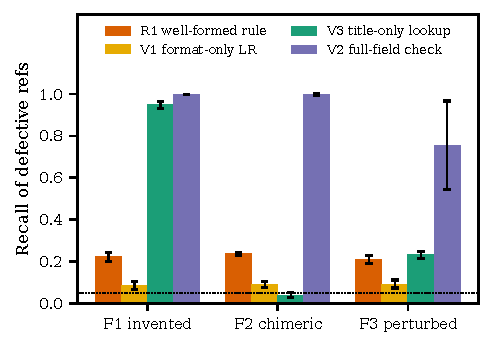
\includegraphics[width=0.93\columnwidth]{figures/fig_recall_by_family}
\caption{Recall of defective references at the 5\%-FPR operating point, by fabrication family (mean $\pm$ SD, 5 seeds). Dotted line: chance (0.05).}
\label{fig:family}
\end{figure}

\begin{table}[t]
\caption{Recall on F3 (perturbed-real) by altered field, $\rho_f{=}0.05$, mean over 5 seeds.}
\label{tab:f3}
\centering\footnotesize
\resizebox{\columnwidth}{!}{\begin{tabular}{@{}lccccc@{}}
\toprule
Verifier & author & year & title & venue/publ. & vol./pages \\
\midrule
V1 format-only LR & 0.102 & 0.095 & 0.114 & 0.048 & 0.101 \\
V3 title-only lookup & 0.020 & 0.041 & 0.846 & 0.036 & 0.009 \\
V2 full-field check & 0.995 & 0.833 & 0.611 & 0.579 & 0.706 \\
\bottomrule
\end{tabular}}
\end{table}

\subsection{Fabricator format fidelity (RQ1 robustness)}
Fig.~\ref{fig:fidelity} shows varying the fabricator's malformation rate. Only the format only models show signal with the fabricator being more sloppy than
the real authors. V1 increases from \NVoneRAuroc{} to \NVoneAurocMid{} and \NVoneAurocHigh{} as $\rho_f$ increases to 0.05, 0.25
and 0.50. The rule R1 also increases to \NRoneAurocHigh{} at 0.50. V2 is relatively unchanged (\NVtwoRAuroc{} to \NVtwoAurocHigh{})
and V3 remains constant around 0.70.

\begin{figure}[t]
\centering
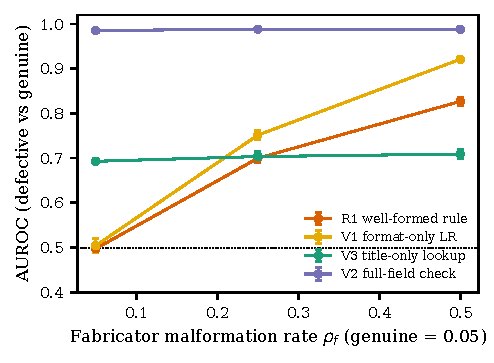
\includegraphics[width=0.93\columnwidth]{figures/fig_fidelity_sweep}
\caption{AUROC (defective vs genuine) as the fabricator's format-malformation rate $\rho_f$ grows; genuine references stay at 0.05.}
\label{fig:fidelity}
\end{figure}

\subsection{Index coverage (RQ3)}
Fig.~\ref{fig:coverage} shows that with thresholds fixed, V2's false-positive rate rises almost exactly as $(1-c)+0.05c$: \NVtwoFprNinety{} at
$c{=}0.9$, \NVtwoFprHalf{} at $c{=}0.5$ and \NVtwoFprQuarter{} at $c{=}0.25$. Recall \emph{rises} (to \NVtwoRecQuarter{} at $c{=}0.25$) only because references whose
true record was removed can no longer be matched and are flagged, so the gain is not detection skill. At an assumed 2\% prevalence the PPV of V2
falls from \NVtwoPpv{} (complete index) to \NVtwoPpvNinety{} (90\%), \NVtwoPpvHalf{} (50\%) and \NVtwoPpvQuarter{} (25\%): nearly every flag is then a false alarm.

\begin{figure*}[t]
\centering
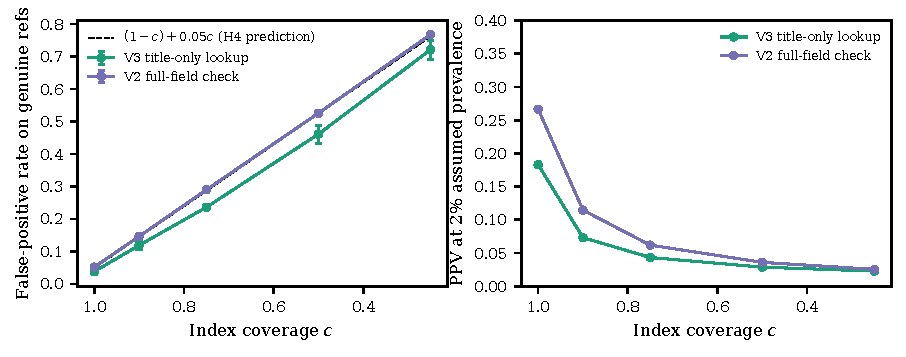
\includegraphics[width=0.78\textwidth]{figures/fig_coverage_sweep}
\caption{Effect of index incompleteness with full-coverage thresholds held fixed. Left: FPR on genuine references; dashed line is the H4 prediction. Right: PPV at 2\% assumed prevalence.}
\label{fig:coverage}
\end{figure*}

\subsection{Error analysis}
V2's F3 recall ranges from \NfthreeMin{} to \NfthreeMax{} depending on seed (SD \NVtwoFthreeSD{}). This can be seen in fig.~\ref{fig:dist} where the
perturbed references that are not author edits have scores of around \NfThreeLo{} to \NfThreeHi{} (middle 50%, seed 0), overlapping with the lower part of real reference scores
(typo + subtitle missing + malformed fields). The author edits have a lower median score (\NfThreeAuthMed{}) and are almost all detected (recall \NVtwoSubAuthor{}).
The 5\%-FPR threshold sits within the overlapping region, ranging from \NtauMin{} to \NtauMax{} depending on seed (see fig.~\ref{fig:tau}). For the seed with the lowest recall (seed \NseedMinRecall{})
\NdegAtMinRecall{}\% of real candidates had scores less than 0.90 so exceeded the 5\% budget. For the other seeds a maximum of \NdegOthersMax{}\% of real candidates had scores below 0.90,
with the F3 recall being at least \NrecOthersMin{}.
This is based on 5 seeds, it was not further tested. Of the \NnFPtotal{} real references that were flagged by V2 in five seeds, \NFPetalPct{}\% were author edits whereby
the author list had been completely ruined (just `et al.'), \NFPtitlePct{}\% were title edits whereby the title had been substantially changed and \NFPotherPct{} just contained some slight
field mismatches.

\begin{figure}[t]
\centering
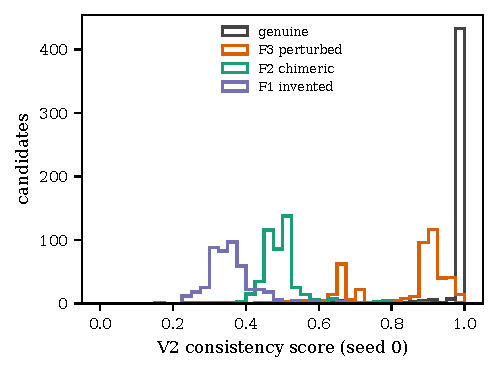
\includegraphics[width=0.93\columnwidth]{figures/fig_v2_score_distributions}
\caption{V2 score distributions by candidate class (seed 0). Perturbed-real references overlap the tail of genuine ones.}
\label{fig:dist}
\end{figure}

\begin{figure}[t]
\centering
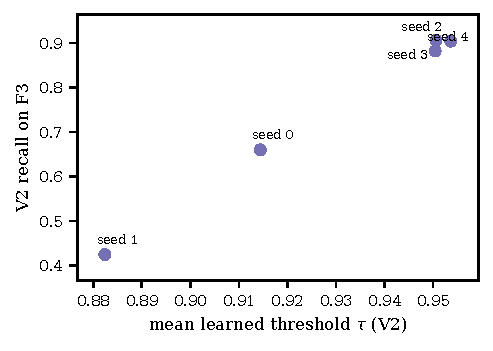
\includegraphics[width=0.93\columnwidth]{figures/fig_tau_vs_f3}
\caption{V2 recall on F3 versus the mean learned threshold $\tau$, one point per seed (exploratory).}
\label{fig:tau}
\end{figure}

\subsection{Outcome of the frozen decision rules}
Table~\ref{tab:hyp} shows that all five pre-specified rules were met. Section~\ref{sec:discussion} explains why that outcome is less informative than it looks.

\begin{table}[t]
\caption{Frozen decision rules and outcomes (mean over 5 seeds).}
\label{tab:hyp}
\centering\footnotesize
\resizebox{\columnwidth}{!}{\begin{tabular}{@{}llcc@{}}
\toprule
ID & Frozen decision rule & Observed & Outcome \\
\midrule
H1 & V1 AUROC at $\rho_f{=}0.05$ in [0.45, 0.60] & 0.504 & supported \\
H1b & V1 AUROC rise (0.05$\to$0.50) $\geq$ 0.15 & +0.417 & supported \\
H2 & V2 recall $\geq$ 0.85 (FPR 5\%, $c{=}1$) & 0.918 & supported \\
H3 & V3 recall $\leq$ 0.20 on F2 and F3 non-title subtypes & max 0.041 & supported \\
H4 & $|$FPR$-[(1{-}c){+}0.05c]|\leq 0.05$ for all $c$ & max dev 0.005 & supported \\
\bottomrule
\end{tabular}}
\end{table}

\section{Discussion}\label{sec:discussion}
\textbf{Designed and informative}. H1, H1b and H4 are all designed to be the results of the simulation. A strict fabricator is
constructed to give no formatting information. A lax fabricator is constructed to give formatting information. Finally, records removed from
a closed-world index cannot be matched, meaning FPR must increase with $1-c$. These are evidence that the pipeline behaves as expected, not that the real world behaves this way. The informative results show (i) there is a large difference between existence and consistency (title-only recall \NVthreeFone{} with fabricated and \NVthreeFtwo{} with chimeric); (ii) the largest errors are near misses (one word changed in title or venue) which are masked by the tolerance required to allow benign typing errors; (iii) the 5\% operating point is unstable where there is as much weight in the true score tail as in the FPR budget; and finally (iv) PPV falls with coverage even when AUROC is high. This means an excellent verifier in the lab can have mostly false alarms in real world conditions.


\textbf{Relation to the review.} These results only support computational claims made in this review within the simulation. This is because there is no information obtained from format-based signals if format faithful forgeries were present. This does not tell us anything about whether people are tricked by format.

\textbf{Practical implications (untested).} Since no record would produce the same result as a forgery, it may be beneficial to report alerts along with coverage of the index. This can be achieved by changing the output to an `uncertain' category rather than a `fabricated' category when there is a `no match'. This was not tested. The PPV here behaves similarly to HALLMARK, in that there is an emphasis on false positive rates \cite{reizinger2026}. However, the values are not comparable.


\section{Deviations from the Frozen Protocol}\label{sec:deviations}
Two issues were identified after the initial frozen run, through analysing results rather than using summary statistics. All nine initial unit tests passed.
\textbf{D1 (parser)} The accent removing regex interpreted the macro \verb|\book{...}| as an accent \verb|\b| character and the letter `o'. This resulted in titles such as
\emph{Narrative of Molloy} being written to 53 out of 468 records as `Narrative of ookMolloy’. \textbf{D2 (label noise)} The F3 perturbations occurred prior to the benign noise meaning that
the field may be reverted by the subsequent noise. 16 out of 468 F3 candidates from seed 0 (3.4%) were identical to the real record but marked as faulty. These were corrected, new regression
tests added and the five seeds ran again with the same decision rules. The results are shown in table ~\ref{tab:prepost}. The most significant change in the metrics is \NmaxDeltaFix{}.
The recall for F3 on V2 decreased from \NpreVtwoFthree{} to \NVtwoFthree{} but no decision rule outcomes changed. As the issues were found by analysing the results, the second run is not blind.

\begin{table}[t]
\caption{Effect of correcting defects D1 and D2 ($\rho_f{=}0.05$, complete index, mean over 5 seeds).}
\label{tab:prepost}
\centering\footnotesize
\begin{tabular}{@{}llccc@{}}
\toprule
Verifier & Metric & Pre-fix & Post-fix & $\Delta$ \\
\midrule
R1 & AUROC & 0.502 & 0.497 & -0.005 \\
R1 & Recall & 0.224 & 0.223 & -0.001 \\
R1 & Recall F3 & 0.221 & 0.210 & -0.012 \\
V1 & AUROC & 0.498 & 0.504 & +0.006 \\
V1 & Recall & 0.084 & 0.089 & +0.005 \\
V1 & Recall F3 & 0.085 & 0.092 & +0.007 \\
V3 & AUROC & 0.700 & 0.693 & -0.007 \\
V3 & Recall & 0.410 & 0.406 & -0.004 \\
V3 & Recall F3 & 0.240 & 0.232 & -0.008 \\
V2 & AUROC & 0.981 & 0.985 & +0.005 \\
V2 & Recall & 0.931 & 0.918 & -0.013 \\
V2 & Recall F3 & 0.796 & 0.756 & -0.041 \\
\bottomrule
\end{tabular}
\end{table}

\section{Threats to Validity and Limitations} \label{sec:threats}
\textit{Fabricated data:} Data is fabricated according to rules rather than an LLM. Realised data may suffer from different artefacts.
\textit{Data Corpus:} A personal bibliography which contains mainly books from the humanities, between the years of \NyearMin{} and \NyearMax{} no DOIs. This makes external validity limited as the review focuses on modern journal references which do contain DOIs. \textit{Ground truth}: Entries are considered real if they appear in the index. No independent verification was carried out.
\textit{Closed world}: There will always be a fully covered entry in the index for a real candidate. However, real databases will have coverage issues and noise.
\textit{Parsing}: Verifiers receive structured data. Parsing errors in the reference strings weren't included in the model.
\textit{Hard-coded weights and perturbations}: Weights in V2 were not tuned. F3 subtypes have equal weighting. In V2, partial credit is given for different venue strings.
\textit{Calibration}: The realised FPR in V1 is higher than 5\%. \textit{Statistics}: Only 5 seeds were used. Standard deviation values were used and no statistical significance was carried out. The $\tau$ was an a posteriori explanation. \textit{Protocol}: The smoke seed was examined before creating the decision rules. Issues D1 and D2 were identified after the first run and resolved (Section~\ref{sec:deviations}). \textit{Baseline}: V2 and V3 were not reproduced versions of published tools. Their numbers should not be interpreted as tool performance.

\section{Conclusion}
Format checks were random in controlled offline simulations (where fabrications were format-accurate), and only improved with increased laxity by fabricators. Title-based existence checks could not detect chimeric or single-field errors. Full-field database consistency detected the majority of errors (e.g. \NVtwoRRec{} had a 5% FPR),
but was dependent on coverage, where the PPV dropped from \NVtwoPpv{} to \NVtwoPpvHalf{}, at 2% prevalence. Next steps would be to
(1) conduct tests on actual LLM fabrications; (2) conduct tests on a modern DOI-containing corpus with a live bibliographic API; and (3) conduct a 3-outcome classification (verified, contradicted, unverifiable) and assess its performance in terms of coverage. The code, protocol, logs and AI assistance log can be found in the associated repository.

\section*{AI-Use Disclosure}
This project was developed using AI assistance (Claude from Anthropic). The AI was used to help plan, write code, debug, write scripts for analysis, create figures and write the report.
All numbers presented here were generated by the publicly available code. The sources were verified from the main pages during the project. The complete prompt and verification can be found in \texttt{ai\_assistance\_log.md}. The contents are the responsibility of the author.
